%%%%%%%%%%%%%%%%%%%%%%%%%%%%%%%%%%%%%%%%%%%%%%%%%%%%%%%%%%%%%%%%%%%%%%%%%%%%%%%%
%2345678901234567890123456789012345678901234567890123456789012345678901234567890
%        1         2         3         4         5         6         7         8

\documentclass[letterpaper, 12 pt, conference]{ieeeconf}  % Comment this line out
                                                          % if you need a4paper
%\documentclass[a4paper, 10pt, conference]{ieeeconf}      % Use this line for a4
                                                          % paper

\IEEEoverridecommandlockouts                              % This command is only
                                                          % needed if you want to
                                                          % use the \thanks command
\overrideIEEEmargins
% See the \addtolength command later in the file to balance the column lengths
% on the last page of the document



% The following packages can be found on http:\\www.ctan.org
\usepackage{graphicx} % for pdf, bitmapped graphics files
\usepackage{bm}
\newcommand{\uvec}[1]{\boldsymbol{\hat{\textbf{#1}}}}
%\usepackage{epsfig} % for postscript graphics files
%\usepackage{mathptmx} % assumes new font selection scheme installed
%\usepackage{times} % assumes new font selection scheme installed
%\usepackage{amsmath} % assumes amsmath package installed
%\usepackage{amssymb}  % assumes amsmath package installed

\title{\LARGE \bf
An Implementation of The ES Algorithm
}

%\author{ \parbox{3 in}{\centering Huibert Kwakernaak*
%         \thanks{*Use the $\backslash$thanks command to put information here}\\
%         Faculty of Electrical Engineering, Mathematics and Computer Science\\
%         University of Twente\\
%         7500 AE Enschede, The Netherlands\\
%         {\tt\small h.kwakernaak@autsubmit.com}}
%         \hspace*{ 0.5 in}
%         \parbox{3 in}{ \centering Pradeep Misra**
%         \thanks{**The footnote marks may be inserted manually}\\
%        Department of Electrical Engineering \\
%         Wright State University\\
%         Dayton, OH 45435, USA\\
%         {\tt\small pmisra@cs.wright.edu}}
%}

\author{Mh. Samadi% <-this % stops a space
}


\begin{document}



\maketitle
\thispagestyle{empty}
\pagestyle{empty}


%%%%%%%%%%%%%%%%%%%%%%%%%%%%%%%%%%%%%%%%%%%%%%%%%%%%%%%%%%%%%%%%%%%%%%%%%%%%%%%%
\begin{abstract}

In this essay we'll go over a basic implementation of the \textbf{Evolutionary Strategy} algorithm that works for any n-dimensional problem. Then we'll define an n-dimensional unimodal test function to test it. The second part of the essay focuses on a technique that will improve the algorithm by orders of magnitude.

\end{abstract}


%%%%%%%%%%%%%%%%%%%%%%%%%%%%%%%%%%%%%%%%%%%%%%%%%%%%%%%%%%%%%%%%%%%%%%%%%%%%%%%%
\section{INTRODUCTION}

In computer science, an evolution strategy (ES) is an optimization technique based on ideas of evolution. It belongs to the general class of evolutionary computation or artificial evolution methodologies.
\\
Evolution strategies use natural problem-dependent representations, and primarily mutation and selection, as search operators. In common with evolutionary algorithms, the operators are applied in a loop. An iteration of the loop is called a generation. The sequence of generations is continued until a termination criterion is met.

\section{Implementation}
The implementation of the algorithm is fairly simple. We start with a random guess that is between +30 and -30 (See ...). The algorithm has a main loop that tries to improve a random guess iteratively.
\\
$X_t$ is the vector of values presented by the algorithm as a guess in t-th iteration of the main loop. In every iteration we'll add a random vector generated based on gaussian normal distribution so that:
\begin{center}
$X_t+1 = X_t + N(0, \sigma)$                    (2.1)
\end{center}
Then the new value will be evaluated and compared to its parent and between these two, the one with the better fitness evaluation (higher value of f (see ...)) will be the parent for the next generation.

\subsection{Test Function}
To evaluate the utility of the algorithm, we'll use the f5 unimodal test function. It is a n-dimensional function that's minimized when the first dimension is 0 (as seen in FIG 1). The f5 function is defined as:
\begin{center}
    $f5(X) = \Sigma_{i=1}^{n-1}(100\times X_{i+1}^2)+(X_i-1)^2$                 (2.2)
\end{center}
The goal is to minimize the output of the test function.
\\
\begin{center}
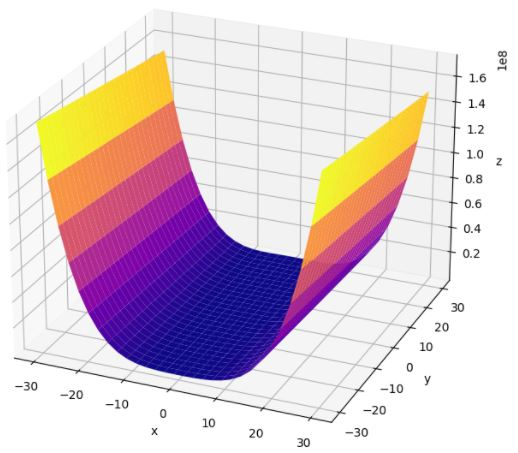
\includegraphics[scale=0.5]{1.JPG}\\
FIG 1. 2D unimodal f5 function
\end{center}

\subsection{Normal Distribution}
The normal distribution seen in 2.1 has a variable $\sigma$ which limits the distance of the possible next guess of the algorithm to the current parent. The algorithm is first ran with a fixed $\sigma$. The results can be seen in .... Then an improvement is made that causes the algorithm to work better by orders of magnitude. The new dynamic $\sigma$ is updated every 10 iterations to try and keep the success rate of the algorithm close to 0.2 (1/5-th rule). 

\section{Results}
The algorithm is ran 3 times in 2, 3, 5, 10, 50 dimensional spaces with and without the improvement made (2.B) for 10000 iterations each. In the 2D setup the results can be visualized:\\
\begin{center}
    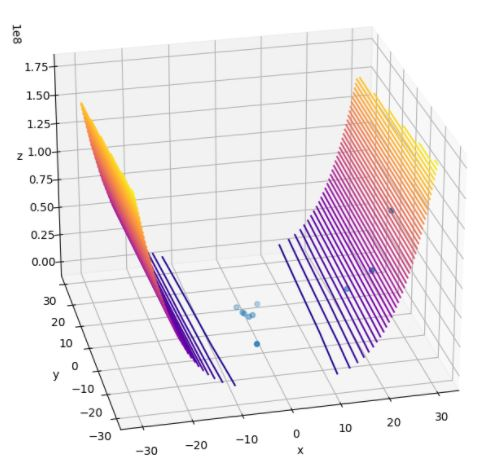
\includegraphics[scale=0.5]{2.JPG}
    \\
    FIG 2. Visualization of the guesses of the algorithm ran with a fixed $\sigma$. The dots represent the different guesses of the algorithm.
\end{center}
As seen in FIG 2, the algorithm with a fixed $\sigma$ has settled on a relatively good point but it's a bit scattered around that point and after the first 4 guesses the final guesses are overshooting and are going back and forth while not getting really better most of the time. But in FIG 3, which shows the results of the improved algorithm with dynamic $\sigma$, the final guesses are converging more gradually towards the final answer and are showing a constant improvement in opposed to getting stuck in a place and depending on a random good guess like the algorithm with a fixed $\sigma$.
\begin{center}
    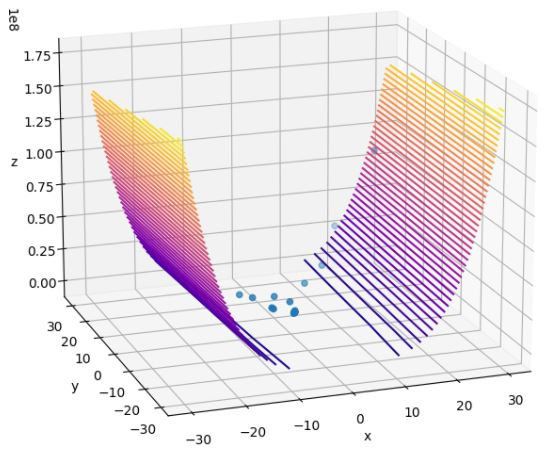
\includegraphics[scale=0.5]{3.JPG}
    \\
    FIG 3. Visualization of the guesses of the algorithm ran with a dynamic $\sigma$. The dots represent the different guesses of the algorithm.
\end{center}
Here are the minimum values the algorithm found for each setup and the number of good guesses that resulted in the creation of a new parent out of 10000 iterations:

\begin{center}
\scalebox{0.7}{
\begin{tabular}{ |c|c c c| } 
 \hline
 - & run 1 & run 2 & run 3\\
 \hline
 2D-Fixed $\sigma$ & 5.2e-6(13) & 4.1e-5(10) & 1.1e-5(10)\\
 2D-Dynamic $\sigma$ & 5.1e-8(23) & 2.3e-8(6) & 1.4e-9(17)\\
 \hline
 3D-Fixed $\sigma$ & 1.55(20) & 8.23(10) & 1.39(18)\\
 3D-Dynamic $\sigma$ & 1.0e-5(44) & 3.68e-5(39) & 3.31e-5\\
 \hline
 5D-Fixed $\sigma$ & 413(22) & 628(21) & 54(9)\\
 5D-Dynamic $\sigma$ & 5.8e-4(96) & 1.5e-5(134) & 2.6e-4(57)\\
 \hline
 10D-Fixed $\sigma$ & 33669(17) & 27842(28) & 7980(25)\\
 10D-Dynamic $\sigma$ & 5.8e-3(1384) & 2752(1642) & 467(637)\\
 \hline
 50D-Fixed $\sigma$ & 26725179(28) & 19798323(36) & 15026812(39)\\
 50D-Dynamic $\sigma$ & 527(1644) & 376(1776) & 18(1760)\\
 \hline
\end{tabular}}
\end{center}

\begin{center}
    FIG 4. Results of running the algorithm multiple times with different dimensionality setups represented in a "best guess(number of good guesses)" format. The improved version of the algorithm increased the number of good guesses and made guesses better by orders of magnitude.
\end{center}

\section{Conclusion}
As seen in FIG 4, the dynamic sigma increases the number of guesses and makes the final answers achieved by the algorithm by orders of magnitude. Overall, the ES algorithm finds a good answer really fast (in 10000 iterations) on a simple test function which shows the utility of the algorithm in simple problems.
\end{document}
